\documentclass[11pt,a4paper]{article}
\usepackage[english]{babel}
\usepackage[utf8]{inputenc}
\usepackage[T1]{fontenc}
\usepackage[top=3.2cm,bottom=2.2cm,left=2cm,right=2cm,headheight=45pt,headsep=0.6cm]{geometry}
\usepackage{graphicx,fancyhdr,xcolor}
\usepackage[hidelinks]{hyperref}
\setlength{\parindent}{0pt}
\setlength{\parskip}{3pt}
\pagestyle{fancy}
\fancyhf{}
\fancyhead[L]{
\includegraphics[width=1.8cm]{img/udglogo.png}}
\fancyhead[C]{\small\textbf{Escola Polit\`ecnica Superior}\\IFRoS / MIRS\\Robot Manipulation}
\fancyhead[R]{\small Lab 2A -- TS60\\Group A}
\fancyfoot[C]{\thepage}
\renewcommand{\headrulewidth}{0.5pt}
\newcommand{\todo}[1]{\textcolor{blue!60!black}{[To complete: #1]}}
\newenvironment{compactitems}{\begin{list}{$\bullet$}{\setlength{\leftmargin}{1.2em}\setlength{\itemsep}{2pt}\setlength{\parsep}{0pt}\setlength{\topsep}{4pt}}\raggedright}{\end{list}}
\begin{document}
\begin{center}
{\LARGE\bfseries Pick and Place with the St\"aubli TS60}\\[6pt]
{\large Lab 2A -- Group A}\\[6pt]
Diego Marzá Fuertes \quad Mario López Honrubia\\
Ismael Bentaleb Ezuitni \quad Antonio Jose Sandoval Hurtado\\[4pt]
\textbf{Highest level demonstrated on the real robot: Level 3}
\end{center}

\section{Task and setup}
We used the St\"aubli TS60 with a suction pad to move metallic and non-metallic cylinders from two ramps to separate groups on a matrix. We programmed the robot in SRS 2019 using VAL3, following the three levels in the lab handout~[1] and the cell shown in Figure~\ref{fig:cell}.

\begin{compactitems}
\item \textbf{Level 1: Basic classification.} One part placed by hand in each ramp, then picked and placed. Two parts in total.
\item \textbf{Level 2: Continuous feeding.} Four parts loaded in each ramp, then picked and placed in repeated cycles. Eight parts in total.
\item \textbf{Level 3: Continuous feeding with automated classification.} Mixed parts loaded in the source tower. The program controls feeding, material detection and sorting until four parts of each material are placed.
\end{compactitems}

\begin{figure}[htbp]
\centering
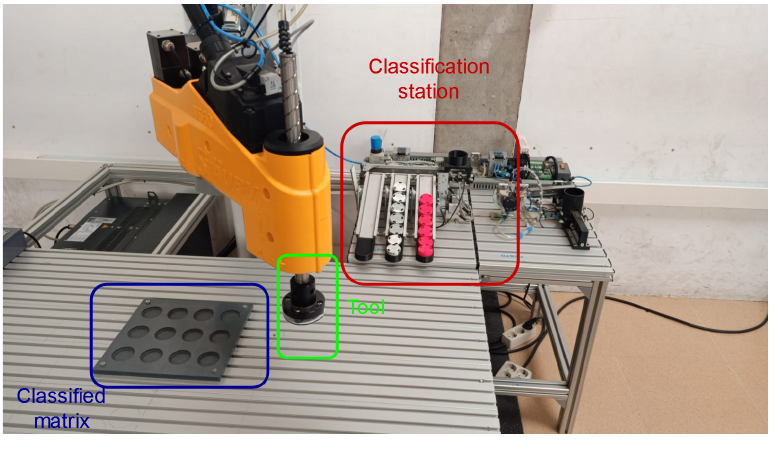
\includegraphics[width=0.65\linewidth]{img/cell-elements.png}
\caption{Classification station, suction tool and destination matrix. Image from the lab handout~[1].}
\label{fig:cell}
\end{figure}

The levels build on the same pickup and placement sequence: Level 1 handles one part from each ramp, Level 2 repeats the operation to fill the matrix, and Level 3 connects this cycle to the feeding and classification station.

\section{Program}
We divided each application into four programs so that the sequence for each level stays in \texttt{start}, while \texttt{pickAndPlace} can be reused for each ramp and destination. In physical mode, \texttt{physicalIO} runs at the same time as the main task to read the sensors and send the output commands, including while \texttt{start} is waiting for a response; \texttt{stop} defines the commands used to end the application.

The cycle uses the same sensor and command variables in simulation and on the real robot, with the \texttt{simulation} flag deciding how they are connected. With \textbf{simulation enabled} (\texttt{true}), we change the sensor variables by hand as the program reaches each wait: \texttt{partOnTool=true} confirms pickup, and \texttt{false} confirms release. For L3 we also choose \texttt{partIsMetal} before confirming \texttt{partAtClass}, then change \texttt{partAtRamp} to represent passage through the ramp sensor; we can see the output variables change, but the program does not send them to the hardware.

With \textbf{physical mode selected} (\texttt{simulation=false}), \texttt{start} creates the \texttt{physicalIO} task, which reads the real inputs into those same variables and applies the program's output commands to the station. This lets us use the same main sequence in both modes: L1/L2 connect the suction tool signals, while L3 also connects the feeding and classification devices. At startup, \texttt{physicalRun = !simulation} stores the choice for the whole run, so changing mode requires stopping and restarting the application.

\begin{figure}[htbp]
\centering
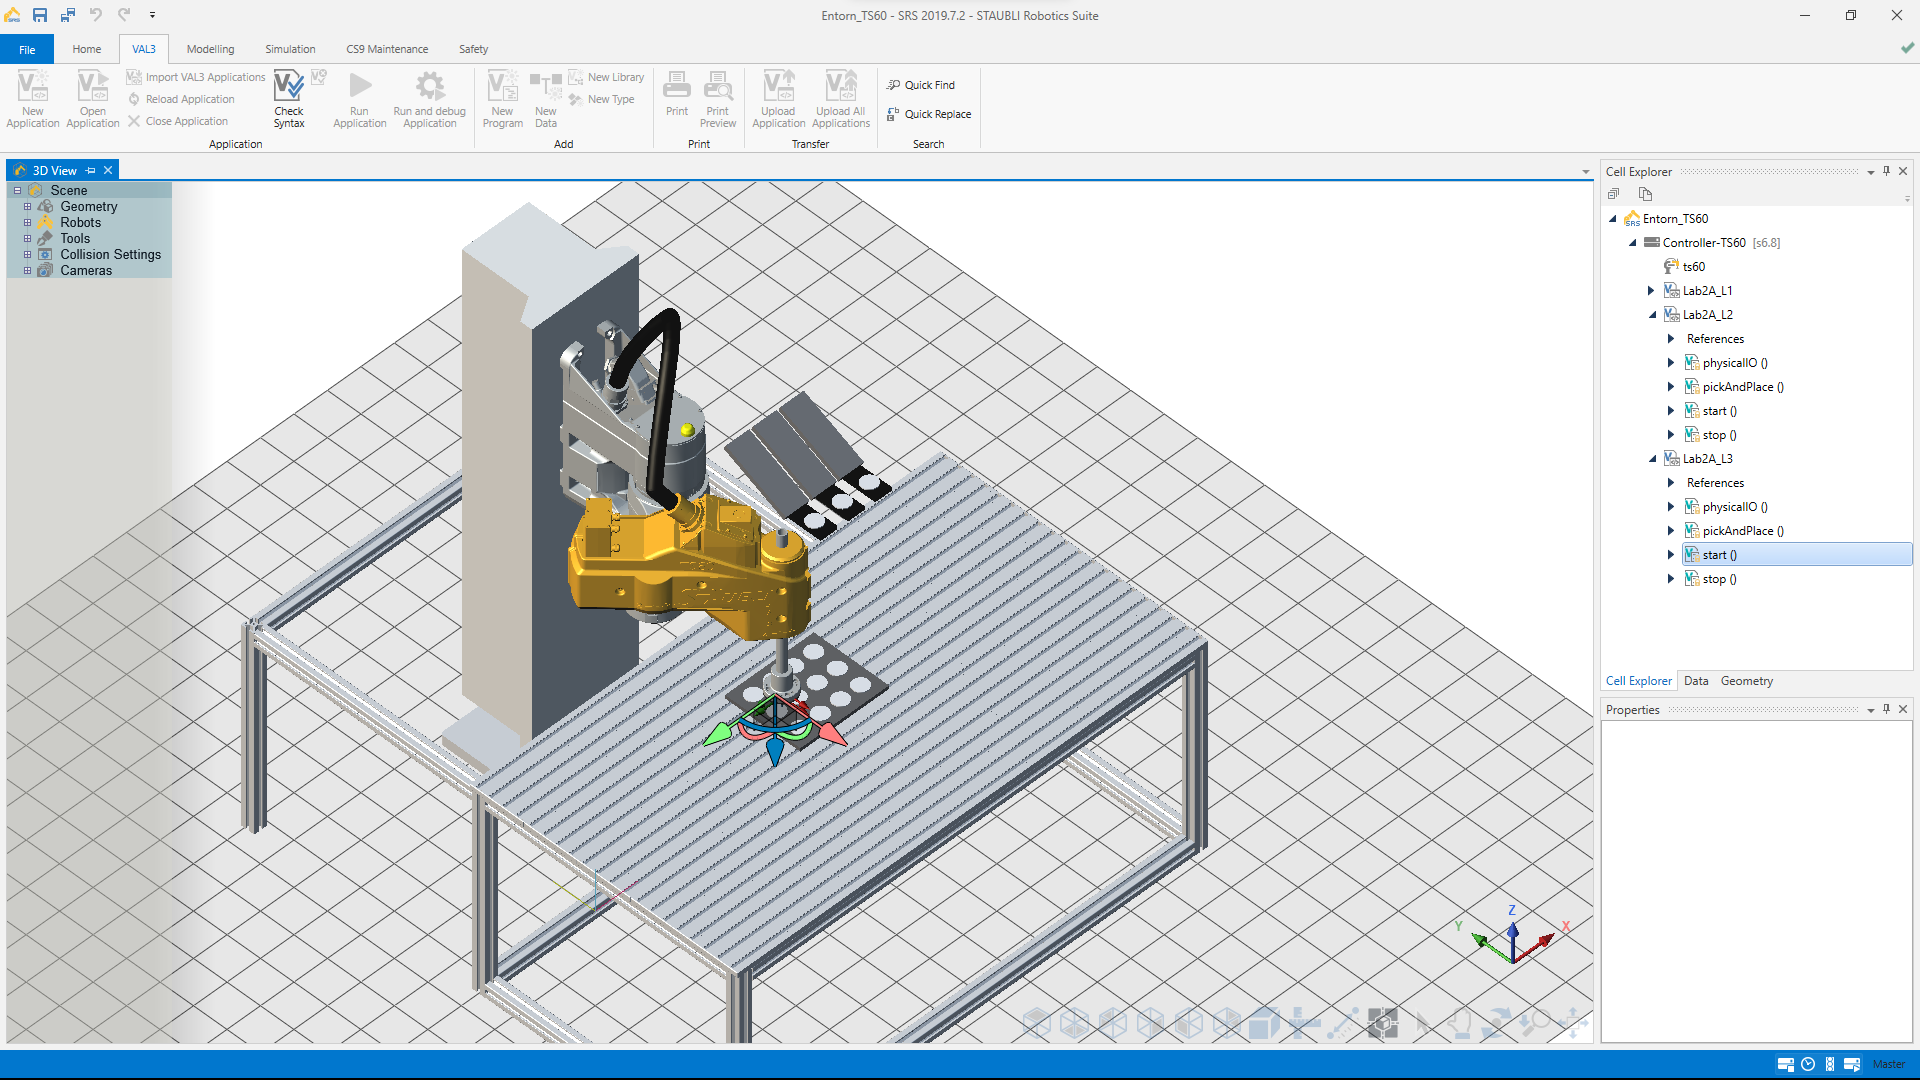
\includegraphics[width=0.95\linewidth]{img/srs-workspace.jpg}
\caption{SRS 2019 workspace with the TS60 scene and the separate L1, L2 and L3 applications in Cell Explorer.}
\label{fig:srs}
\end{figure}

\subsection{Pick and place}
To pick up a part, the robot first moves to the approach position above the ramp with \texttt{movej}, then moves down to the pickup position with \texttt{movel} and turns on suction. It waits for \texttt{partOnTool=true} before moving back up, so it only starts moving towards the destination after the sensor confirms that it holds a part. At the destination, the robot moves down from the approach position, turns off suction and blows air for 0.3\,s to release the part; once \texttt{partOnTool=false} confirms that it is released, the robot moves back up and returns home.

We use \texttt{movej} to move between approach positions and \texttt{movel} to move in a straight line near the parts. After each move, \texttt{waitEndMove()} makes the program wait until the robot finishes moving before it runs the next command, such as turning on suction or releasing the part.

\subsection{Level 1: Basic classification}
For basic classification, we place one cylinder in each ramp and use two taught destinations, with index 0 for non-metallic and 1 for metallic. After calculating an approach 50\,mm above each destination, \texttt{start} selects the ramp and matching destination and calls \texttt{pickAndPlace}, completing the same operation once for each material.

\subsection{Level 2: Continuous feeding}
Level 2 extends this sequence to four parts per ramp, keeping the two taught reference positions as slots 0 and 4 and calculating the other positions along each material group. A loop alternates the ramps and fills slots in the order \texttt{0,4,1,5,2,6,3,7}; because the number and order of pickups are fixed, the loop indices also give us the next destination. As in Level 1, we load the ramps before starting and the program uses only the suction sensor, vacuum and blow outputs.

\subsection{Level 3: Continuous feeding with automated classification}
In Level 3, the feeding station sends the parts while the conveyor keeps running. Once the sensor detects a part at the classification station, the program reads the inductive sensor, stores the material as 0 or 1 and selects the matching sorting actuator. After waiting 0.5\,s for the actuator to move, it opens the barrier for 0.4\,s and closes it again, then waits for the ramp sensor to turn on and then off as the part passes. Physical mode includes another 0.5\,s delay to allow the part to reach the pickup location.

Each material has its own counter. The next destination is
\[
\texttt{placeIndex}=4\,\texttt{materialType}+\texttt{placedCount[materialType]}.
\]
The counter increases after \texttt{pickAndPlace} returns, which lets the next part of that material use the following free destination whatever order the parts arrive in. If its group already contains four parts, the program skips pickup and continues looking for the material still needed; these extra parts remain in their ramp. Once both counters reach four, the program stops the conveyor and leaves the barrier closed.

\textbf{Level 3 sequence:}
\begin{enumerate}
\setlength{\itemsep}{1pt}
\setlength{\parsep}{0pt}
\item Prepare geometry and I/O, start the conveyor and move home.
\item Wait for classification presence and store the material.
\item Select the sorting actuator, open and close the barrier, then wait for the part to pass the ramp sensor.
\item Pick and place if that material still has a free slot, then add one to its counter.
\item Repeat from step 2 until both counters reach four. Stop the conveyor and keep the barrier closed.
\end{enumerate}

\section{Parameters and data}
We define the application positions relative to \texttt{world}, with zero translation and rotation, and define the suction TCP at an offset of \texttt{(0,20,0)}\,mm from \texttt{flange}, also with zero relative rotation. The tool uses the local \texttt{toolDummy} as its I/O reference because the cycle controls vacuum and blow through separate output commands rather than \texttt{open()} and \texttt{close()}.

\begin{compactitems}
\item \textbf{Motion:} \texttt{moveSpeed} has velocity, acceleration and deceleration set to 10, with blending off. \texttt{tmax=rmax=99999} are the original motion descriptor values, not measured operating speeds.
\item \textbf{Geometry:} placement approaches are world Z +50\,mm above the destination. L2/L3 columns are spaced by world Y +60\,mm from each material's taught reference.
\item \textbf{Timing:} blow pulse 0.3\,s. L3 uses 0.5\,s for the sorting actuators, a 0.4\,s barrier opening and 0.5\,s of extra waiting time at the ramp in physical mode.
\end{compactitems}

The matrix calculation in L2 and L3 starts from the taught reference for each material, at slots 0 and 4. We convert each reference to Cartesian coordinates with \texttt{jointToPoint}, apply the column offset and pass the result to \texttt{pointToJoint} to get the next joint position. This also gives us a check before starting the cycle: the program exits if a destination or approach cannot be calculated, although we still need to check the path even if the calculation succeeds.

The taught joint values below use degrees for J1, J2 and J4, and millimetres for J3:
\begin{compactitems}
\item \textbf{Home:} \texttt{(0, 0, 150, 0)}.
\item \textbf{Pickup:} non-metallic \texttt{(59.97, 53.21, 23.19, -318.70)}; metallic \texttt{(47.65, 78.71, 25.69, -318.70)}.
\item \textbf{Destination references:} non-metallic \texttt{(-88.79, 115.82, 6.90, 1.55)}; metallic \texttt{(-77.39, 100.14, 8.89, -353.18)}.
\end{compactitems}
The pickup approaches keep the same J1, J2 and J4 values and raise J3 to 100\,mm, while the placement approaches and remaining matrix destinations are calculated at startup. Their initial values in the data file are placeholders, rather than the final positions used during the cycle. No payload measurement is included in our notes.

\subsection{Variables and I/O}
Array sizes are shown in brackets; other data contain one element.

\begin{compactitems}
\item \textbf{Mode and I/O setup:} \texttt{simulation}, \texttt{physicalRun} and \texttt{ioReady} are booleans for the chosen mode, the stored mode and completion of the first I/O update.
\item \textbf{Suction tool:} \texttt{partOnTool} reads \texttt{bIn0}; \texttt{vacuumOn} and \texttt{blowOn} command \texttt{bOut0} and \texttt{bOut1}. All three are booleans.
\item \textbf{Selection:} \texttt{materialType} is numeric, with 0 for non-metallic and 1 for metallic. Numeric \texttt{placeIndex} selects destination 0--1 in L1 or 0--7 in L2/L3.
\item \textbf{Status:} numeric \texttt{cycleStep} records 60 for grip, 70 for release, 100 for completion and -1 for stop. L3 also uses steps 20--50 and 80.
\item \textbf{Joint poses:} \texttt{homePose} is the home position. \texttt{pickPose[2]} and \texttt{pickApproach[2]} hold the two ramp poses and approaches. \texttt{placePose} and \texttt{placeApproach} have size 2 in L1 and size 8 in L2/L3. All are \texttt{jointRs} data.
\item \textbf{References and motion:} \texttt{world} is a frame; \texttt{flange} and \texttt{vacuumTool} are tools. \texttt{moveSpeed} is an \texttt{mdesc}; \texttt{toolDummy} is a local unlinked \texttt{dio}.
\end{compactitems}

\begin{samepage}
\textbf{Level 3 adds:}
\begin{compactitems}
\item \textbf{Classification sensors:} booleans \texttt{partAtClass}, \texttt{partIsMetal} and \texttt{partAtRamp} read the part sensor \texttt{bIn1}, the inductive sensor \texttt{bIn2} and the ramp sensor \texttt{bIn4}.
\item \textbf{Station commands:} booleans \texttt{trolleyOn}, \texttt{nonMetalGate} and \texttt{metalGate} control conveyor \texttt{bOut2} and sorting actuators \texttt{bOut3}/\texttt{bOut4}. Boolean \texttt{barrierClosed} uses the opposite output value: \texttt{bOut5 = !barrierClosed}.
\item \textbf{Counters:} numeric \texttt{placedCount[2]} stores the completed placements per material and is reset at startup.
\end{compactitems}
\end{samepage}

\texttt{targetPose} is a local \texttt{pointRs} for geometry calculations. L2/L3 also have local numeric \texttt{rowIndex}, \texttt{columnIndex} and \texttt{targetIndex}. All have size 1. The alias \texttt{io} loads the controller I/O library. L3 leaves \texttt{bIn3} and sorting actuator end switches \texttt{bIn5--bIn8} unused.

\section{Safety and limitations}
The approach positions keep the tool above the parts while it moves between the ramp and the matrix, with straight movements down and back up near each part. We also use a high home position, but we still need to check the complete paths through the cell because reaching the correct position does not mean that the path is safe. The saved program velocity is 10; the lab instructions set a maximum programmed velocity of 30 and ask us to start with the MCP speed override at 10\%~[1].

When the application stops, \texttt{stop} cancels the remaining movements and turns off the air blow, while keeping suction on if it was already on so that the stop command does not release a part. L3 also stops the conveyor and closes the barrier to hold back the next parts. Before starting again, the matrix must be empty because the program resets its counters and does not remember which holes were already filled.

The current sequence uses sensor waits without timeouts and fixed delays for the station actuators, so a missing signal can leave it waiting and a delay alone does not confirm that a sorting actuator reached its position. There are also two timing limits in L3: a ramp pulse can be missed if it begins and ends during the 0.4\,s barrier opening, and the main task can read the previous material value because the I/O task updates presence before the inductive reading. Grip is checked at pickup, but a part lost during transfer could still be counted at the end.

\section{Execution results}
Level 3 was demonstrated on the real robot, and its operation in simulation is available in the \href{https://ugirona-my.sharepoint.com/:v:/g/personal/u6120632_udg_edu/IQCCHUXZbpDZQJx1GxVThgnPAUpKyrIblhpKYQN-_18FjhU?e=oOMlbG}{Level 3 simulation video}. \todo{add the real-execution video and check that the teacher can open both links.}

The syntax check shows zero errors for L1 and L2, so the compiler accepts both programs. We still need to test them in simulation to check the paths and make sure the robot picks up and places the parts as expected. \todo{record the L1/L2 simulation results and videos, and repeat Check Syntax after further code changes.}

During development, the first Cartesian offset did not give us a valid second matrix reference, so we used a taught reference for each material and set the column offset along world Y positive. For the automatic station, we also inverted the barrier output and adjusted its opening to 0.4\,s. We kept these settings in L3, although our notes do not include cycle-time measurements or repeated-run success rates.

\section{Improvements}
The first improvement would be to keep a record of the ramp sensor signal until the main task reads it, and to wait for a stable material reading after a part is detected. This would help avoid the timing problems described above. We would then use the sorting actuator end switches, add time limits to the sensor waits and check that the robot still holds the part before releasing it. These changes would be made in the station and I/O code, while keeping the same pickup and placement routine for all three levels.

\begin{thebibliography}{1}
    \bibitem{lesson} Robot Manipulation, \emph{Pick and Place with the St\"aubli TS60}, lab handout, sections 2--4.
    \end{thebibliography}

\clearpage
\appendix
\section{VAL3 programs}
\todo{Insert the final, checked code after the applications are finished.}

\subsection{Level 1: start}
\todo{Level 1 main program.}

\subsection{Level 2: start}
\todo{Level 2 main program.}

\subsection{Levels 1 and 2: shared routines}
\todo{Final pickAndPlace, physicalIO and stop programs.}

\subsection{Level 3: start}
\todo{Level 3 main program.}

\subsection{Level 3: supporting routines}
\todo{Final pickAndPlace, physicalIO and stop programs.}
\end{document}
